\section{App diagrams}\label{app:app-diagram}
\begin{landscape}
   \begin{figure}
    \centering
    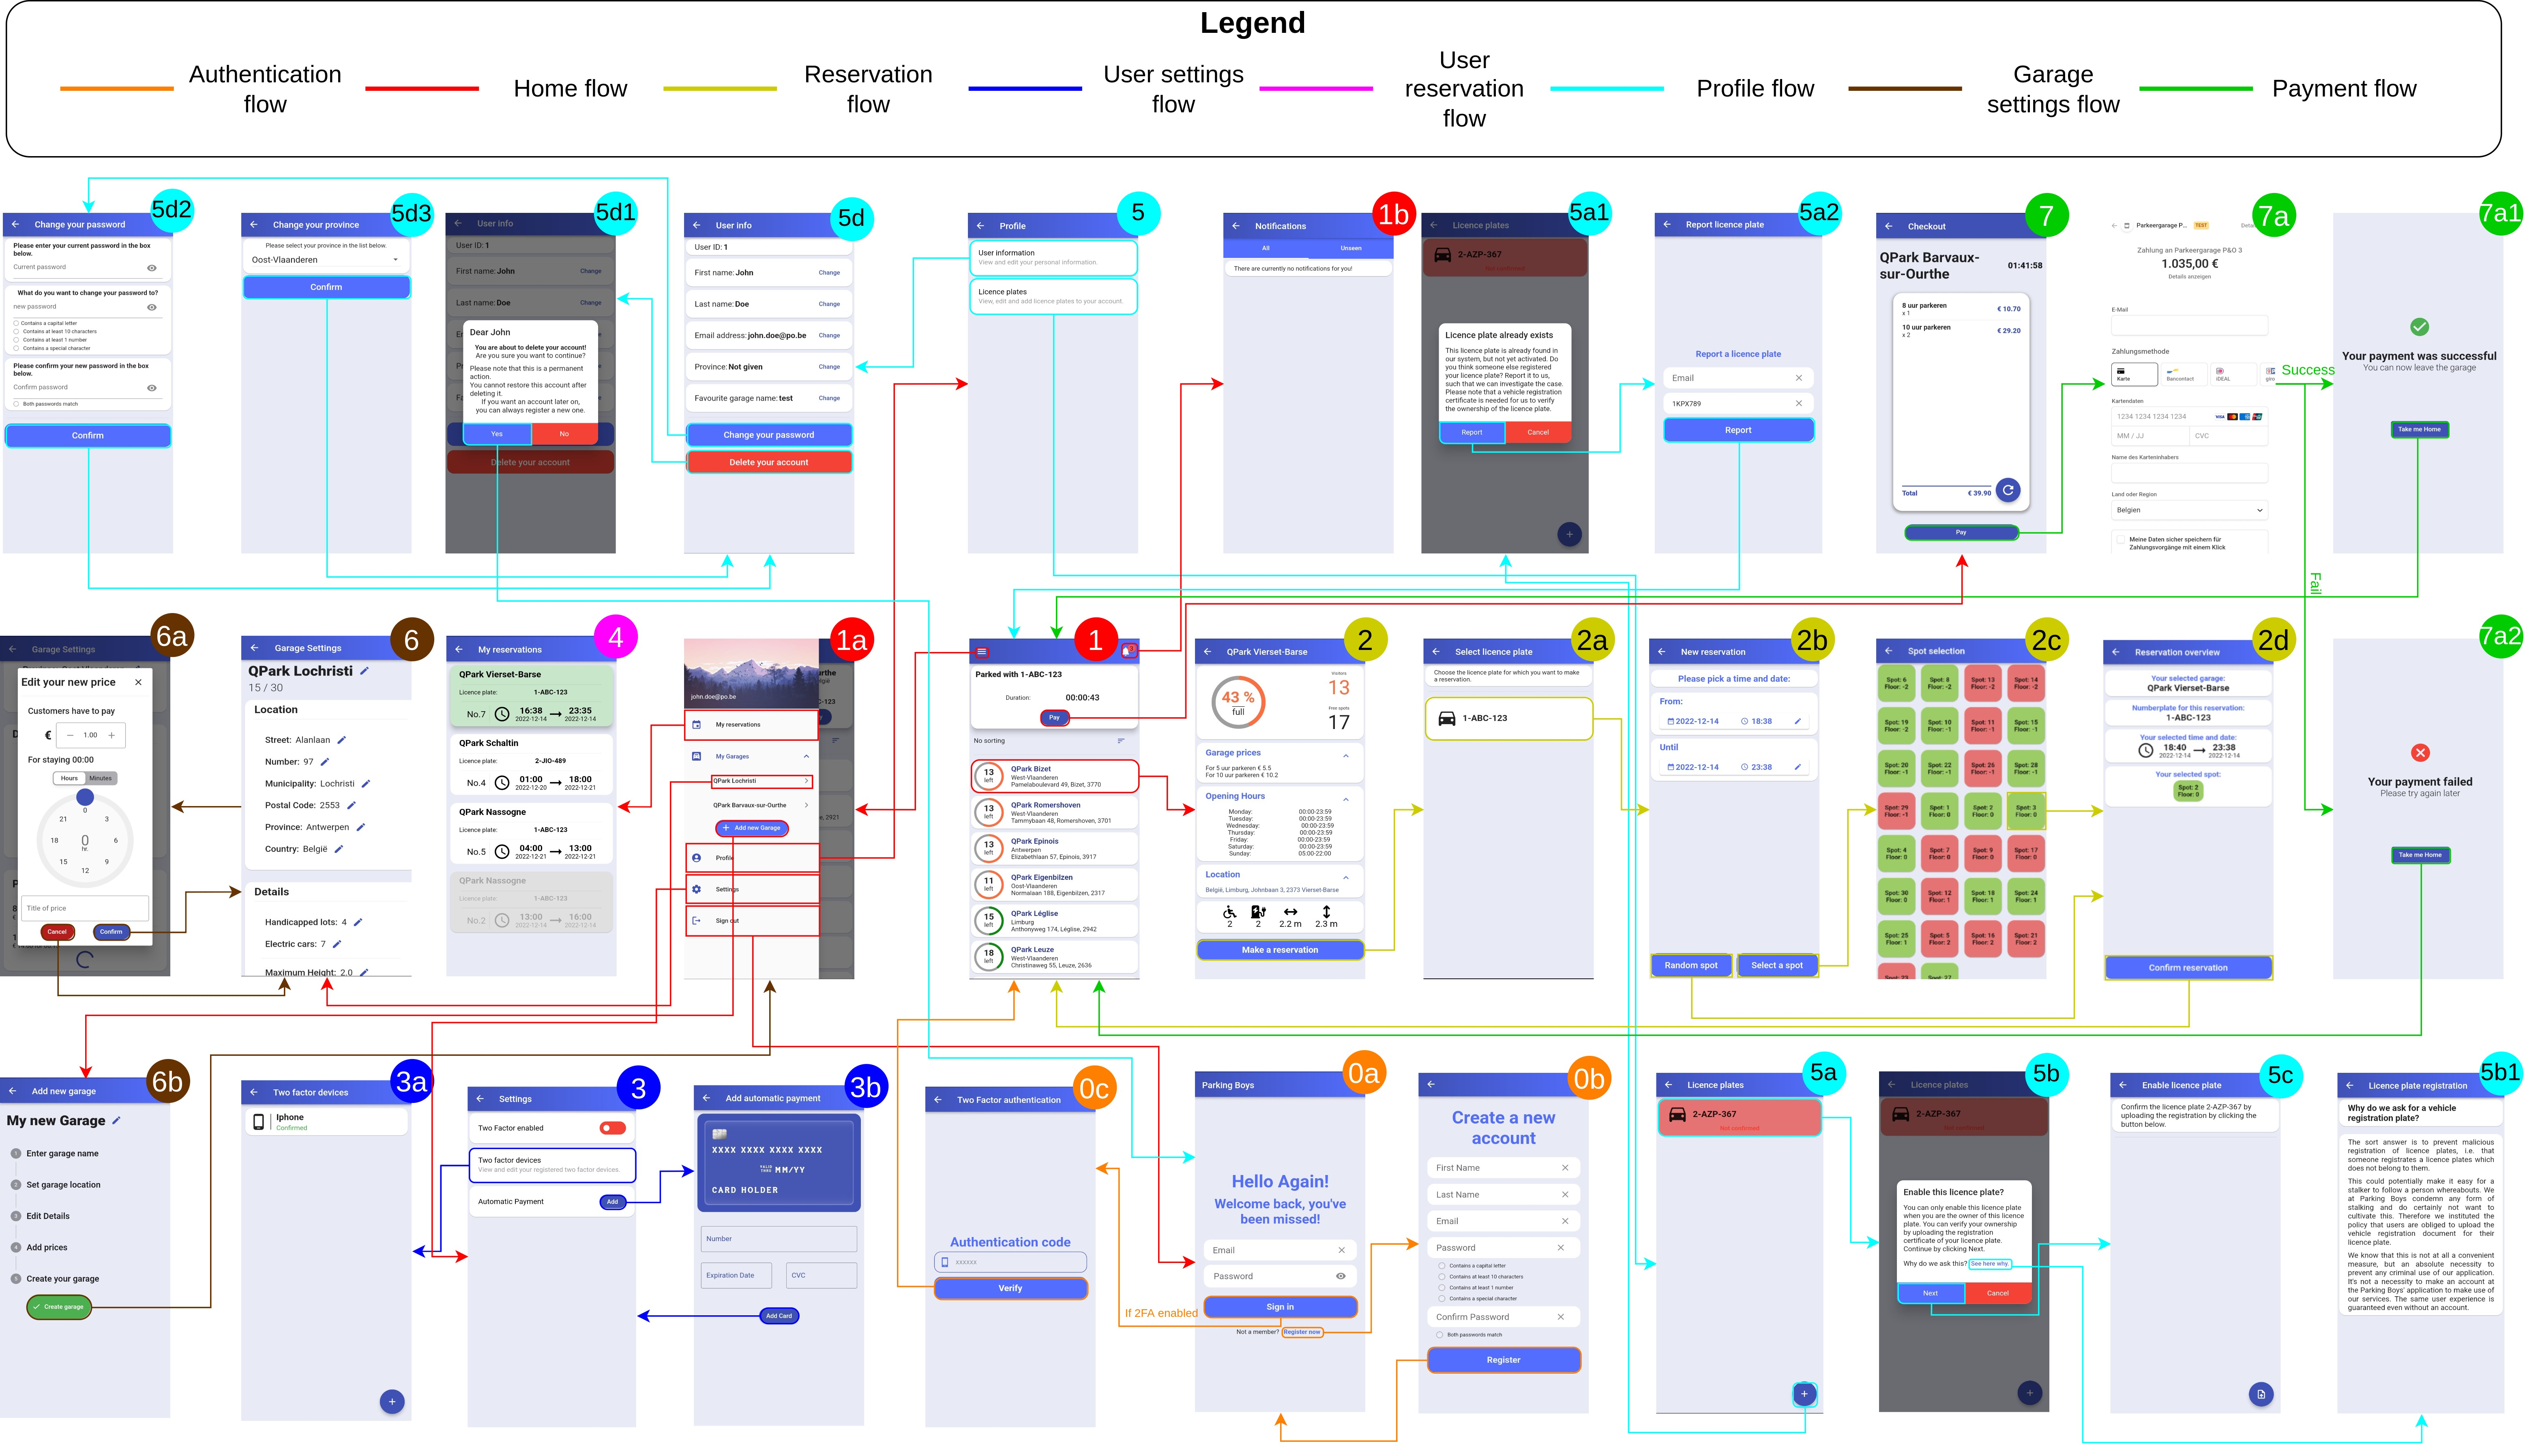
\includegraphics[width=25cm]{images/app/app_diagrams/app_diagram-general.jpg}
    \caption[General app diagram.]{General app diagram which displays the user flow within the frontend application. The pages are enumerated, where a new number indicates a change of flow. Pages with the same number belong to the same logic flow within the application. The routes of the back button are not indicated with an arrow as they represent the reverse direction of the arrow which points to this page.}
    \label{fig:general-app-diagram}
\end{figure}
\end{landscape}

\clearpage
\begin{figure}[hpt]
    \centering
    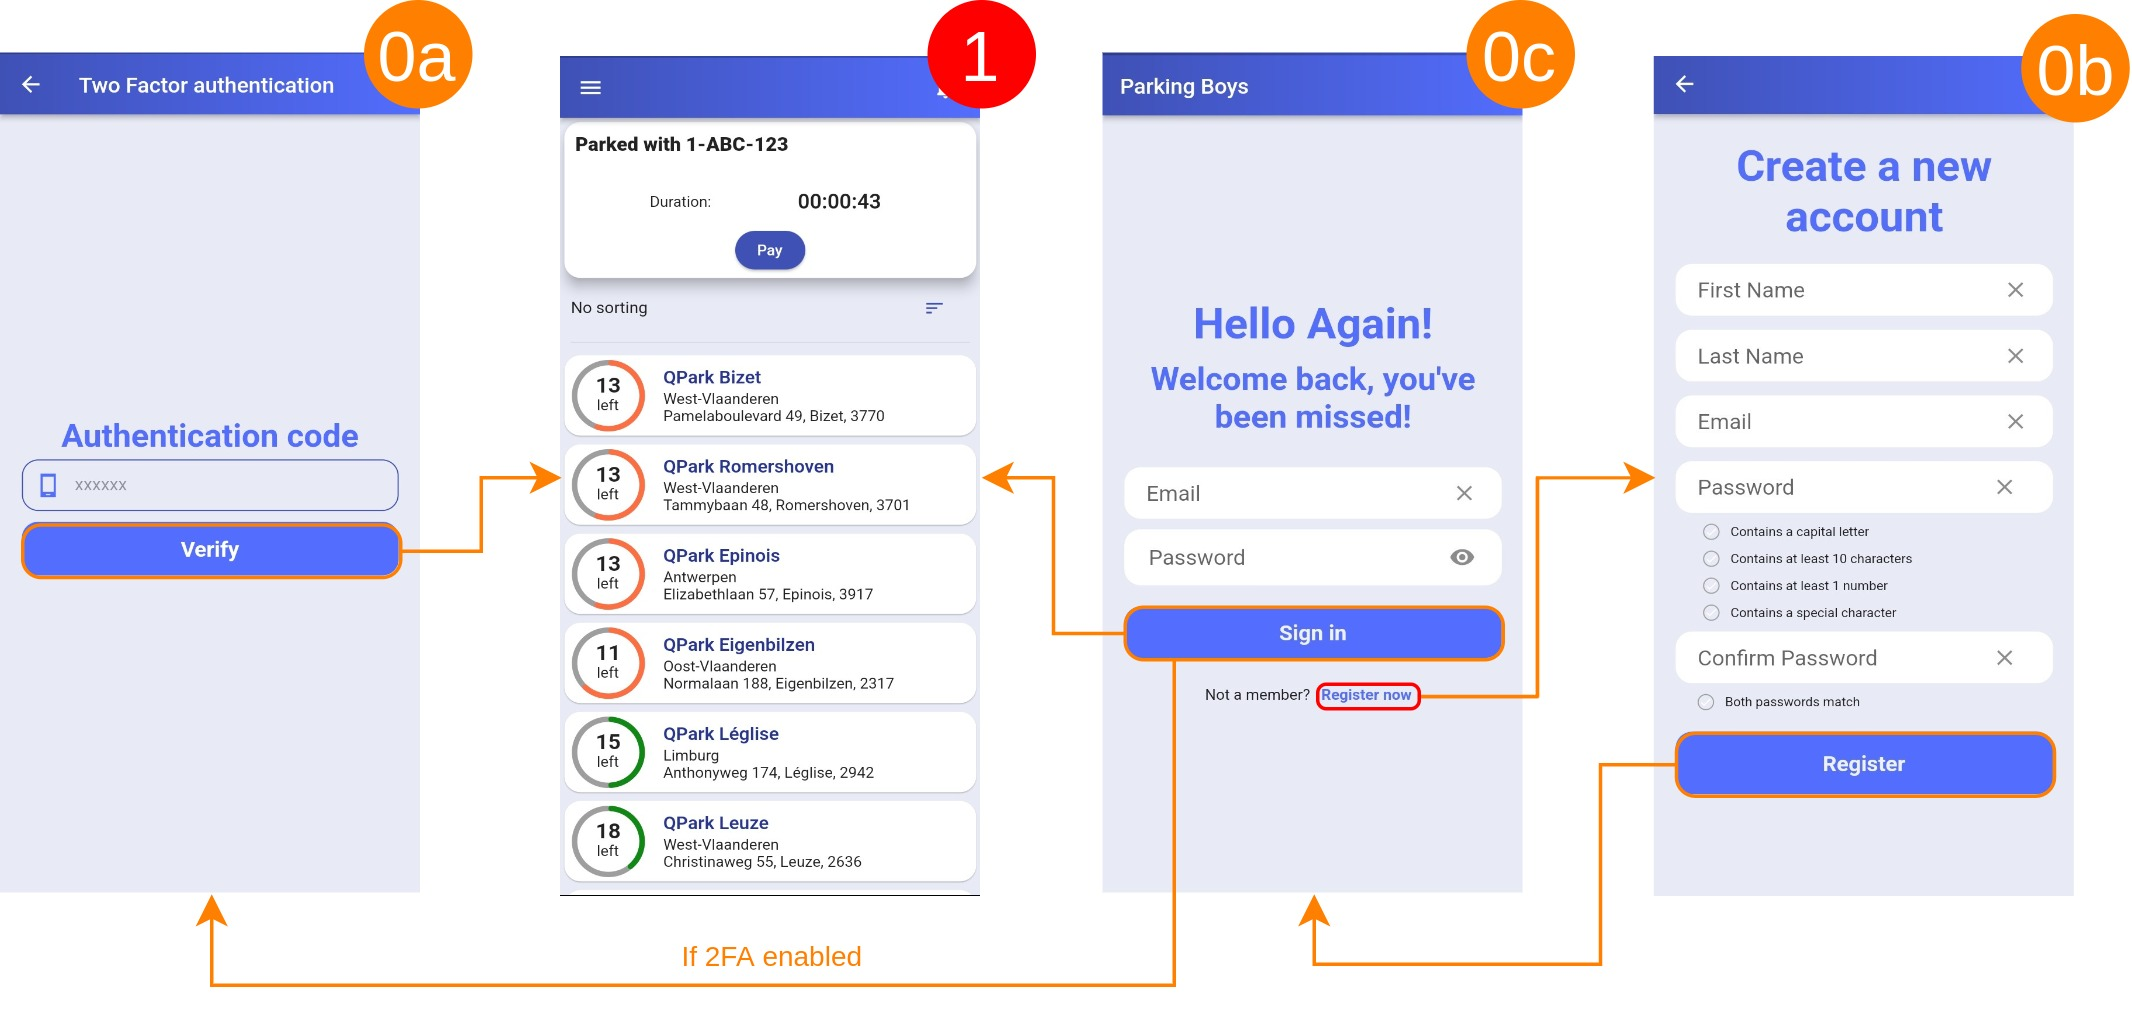
\includegraphics[width=16cm]{images/app/app_diagrams/app_diagram-auth-flow.jpg}
    \caption{App diagram of the authentication flow (Flow 0).}
    \label{fig:auth-flow}
\end{figure}
\begin{figure}[hpt]
    \centering
    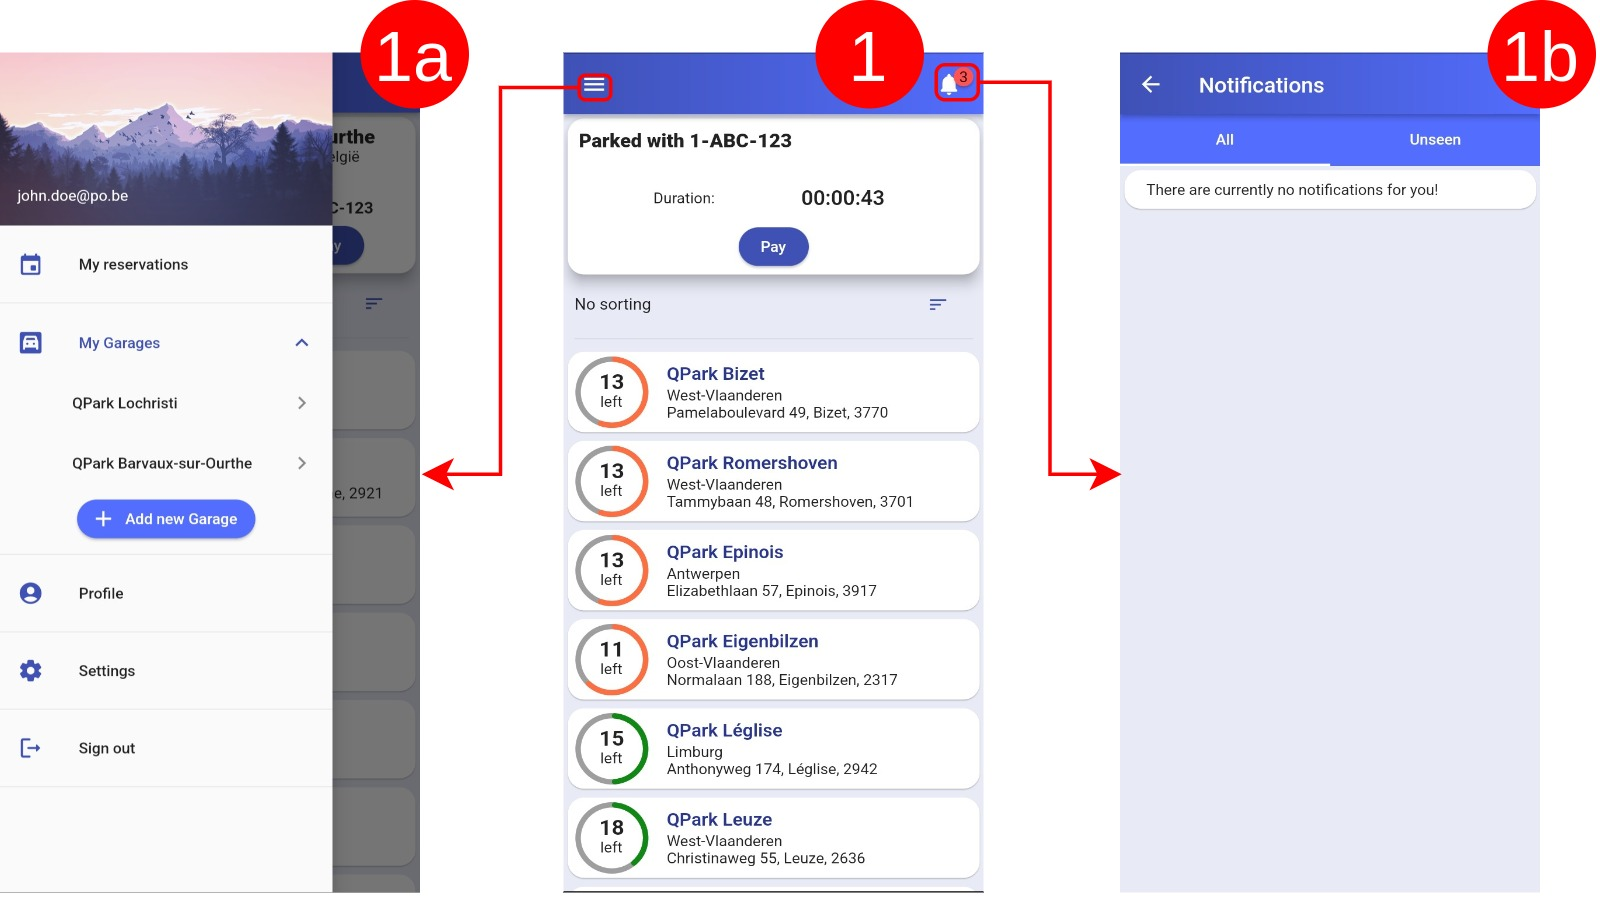
\includegraphics[width=16cm]{images/app/app_diagrams/app_diagram-home-flow.jpg}
    \caption{App diagram of the home flow (Flow 1).}
    \label{fig:home-flow}
\end{figure}

\clearpage

\begin{figure}[hpt]
    \centering
    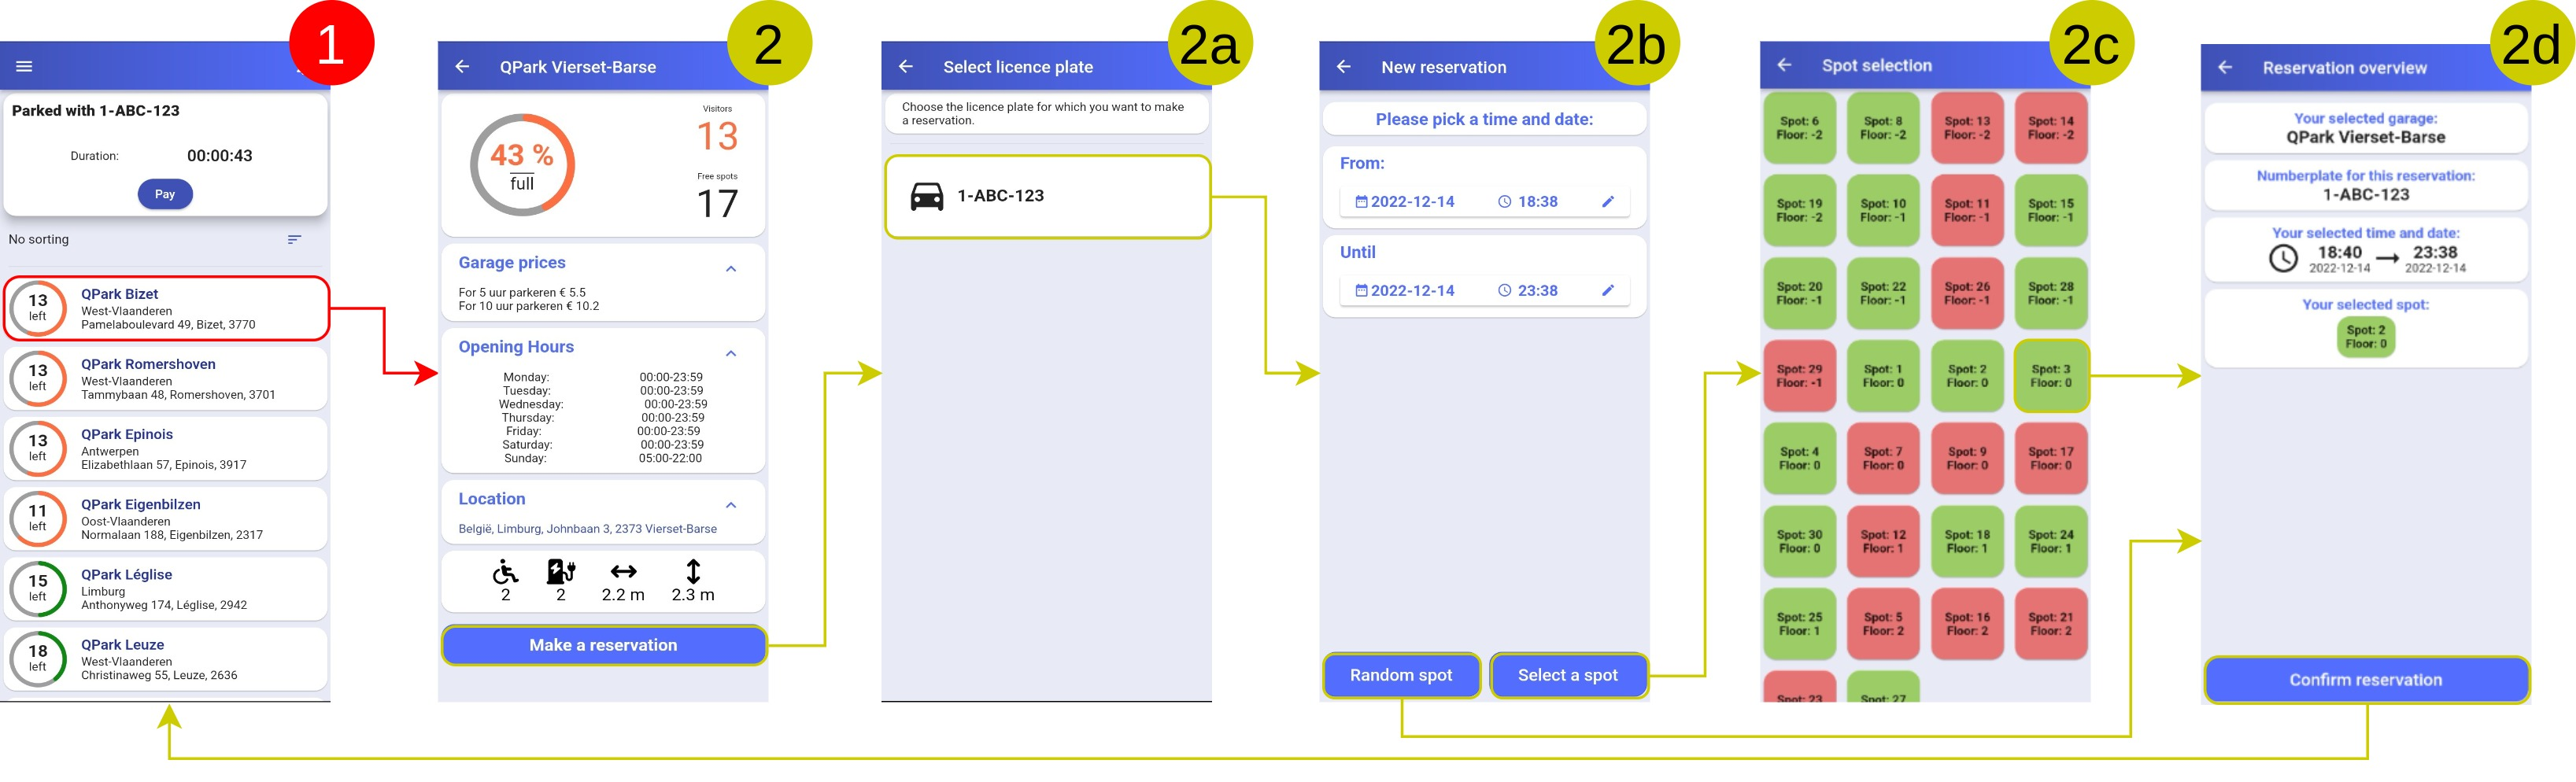
\includegraphics[width=14cm]{images/app/app_diagrams/app_diagram-reservation.jpg}
    \caption{App diagram of the reservation flow (Flow 2).}
    \label{fig:reservation-flow}
\end{figure}
\begin{figure}[hpt]
    \centering
    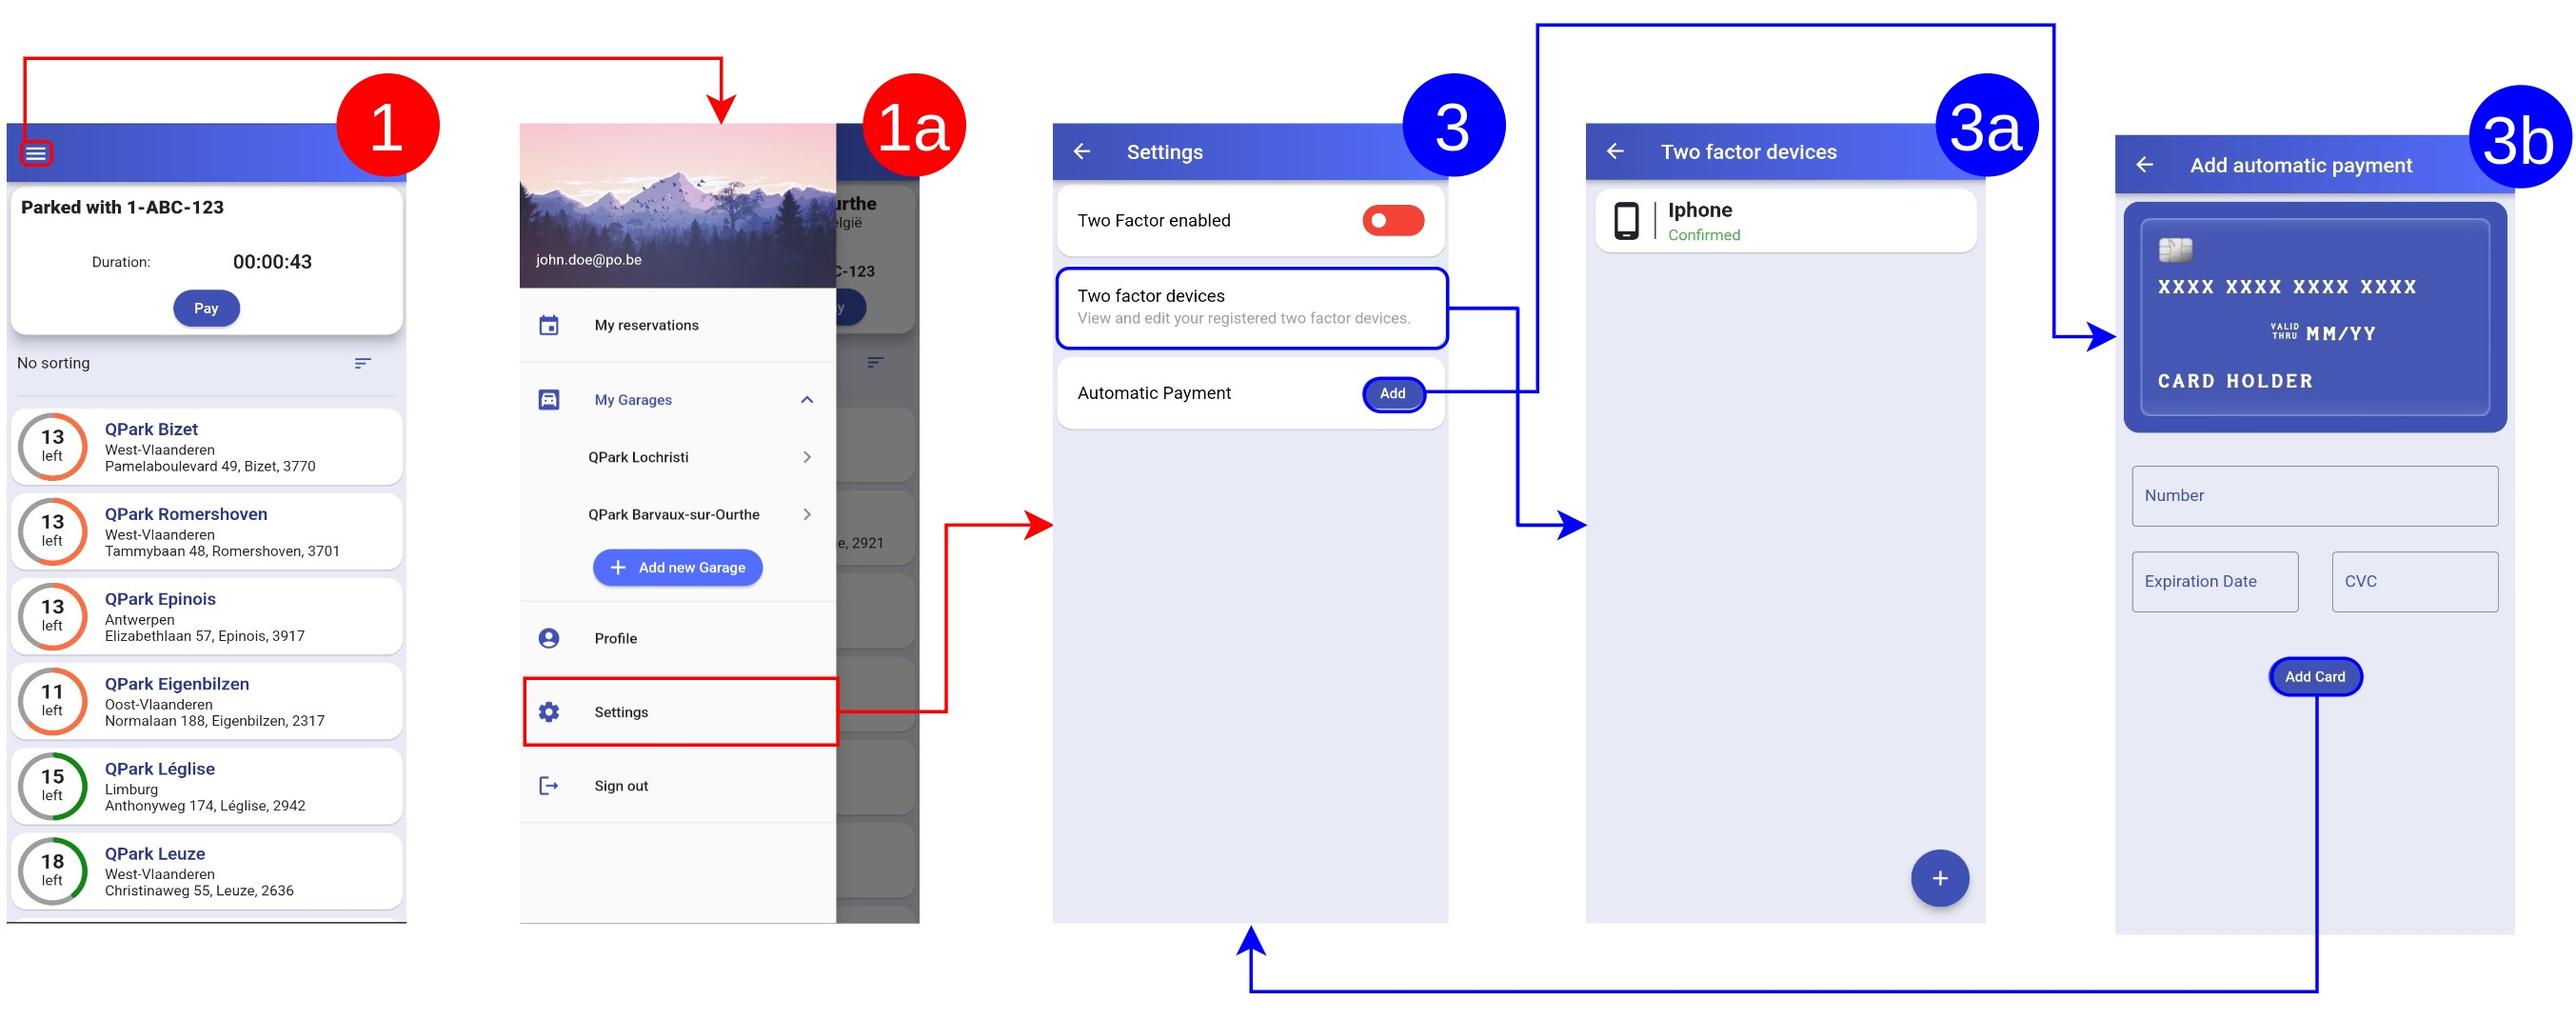
\includegraphics[width=14cm]{images/app/app_diagrams/app_diagram-user-settings-flow.jpg}
    \caption{App diagram of the user settings flow (Flow 3).}
    \label{fig:user-settings-flow}
\end{figure}
\begin{figure}[!hpt]
    \centering
    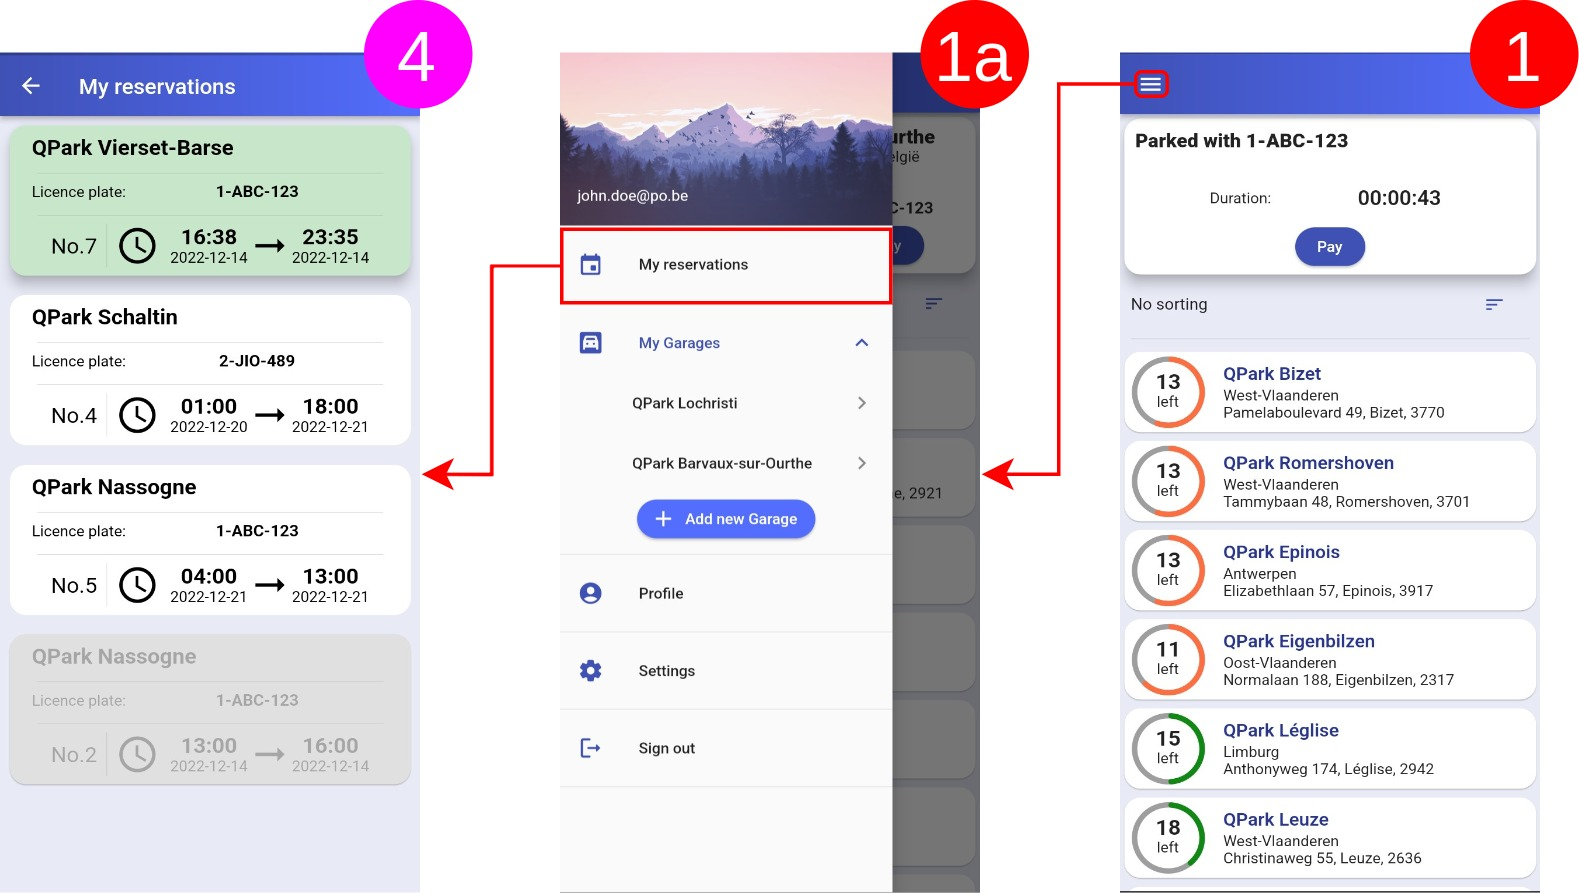
\includegraphics[width=14cm]{images/app/app_diagrams/app_diagram-user-reservation-flow.jpg}
    \caption{App diagram of the user reservation flow (Flow 4).}
    \label{fig:user-reservation-flow}
\end{figure}

\clearpage

\begin{figure}[hpt]
    \centering
    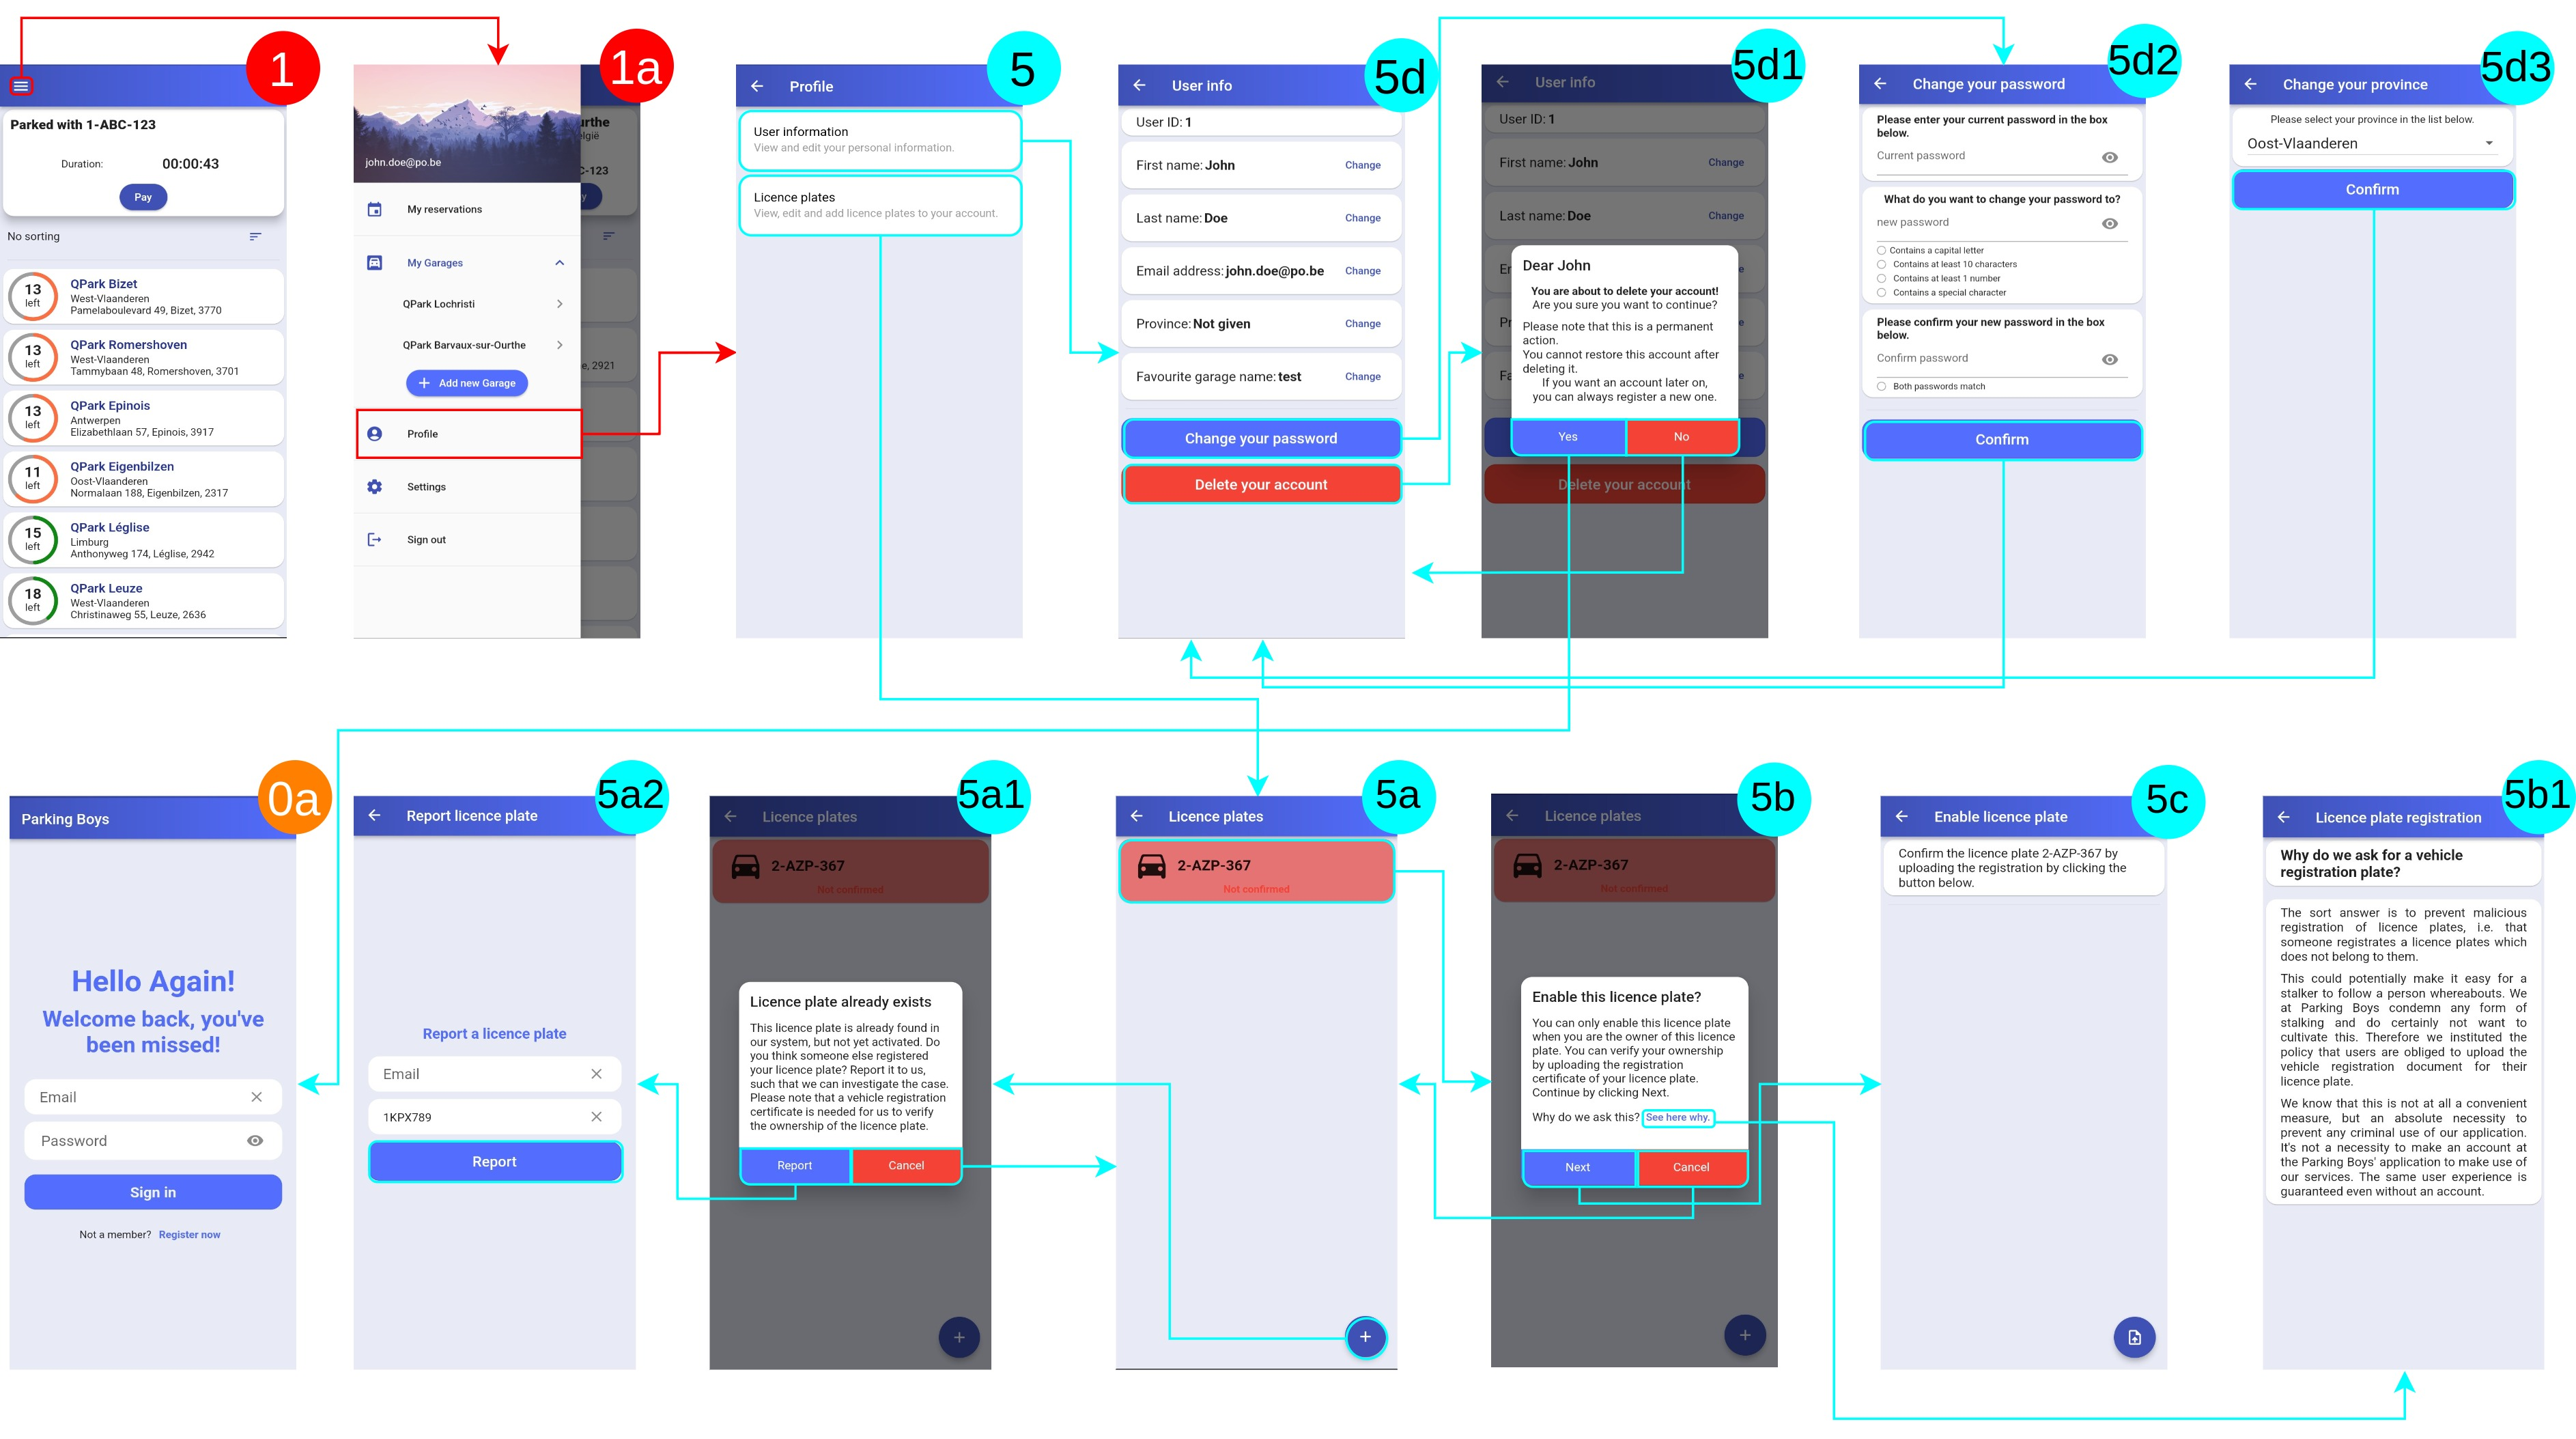
\includegraphics[width=16cm]{images/app/app_diagrams/app_diagram-profile-flow.jpg}
    \caption{App diagram of the profile flow (Flow 5).}
    \label{fig:profile-flow}
\end{figure}
\begin{figure}[hpt]
   \centering
   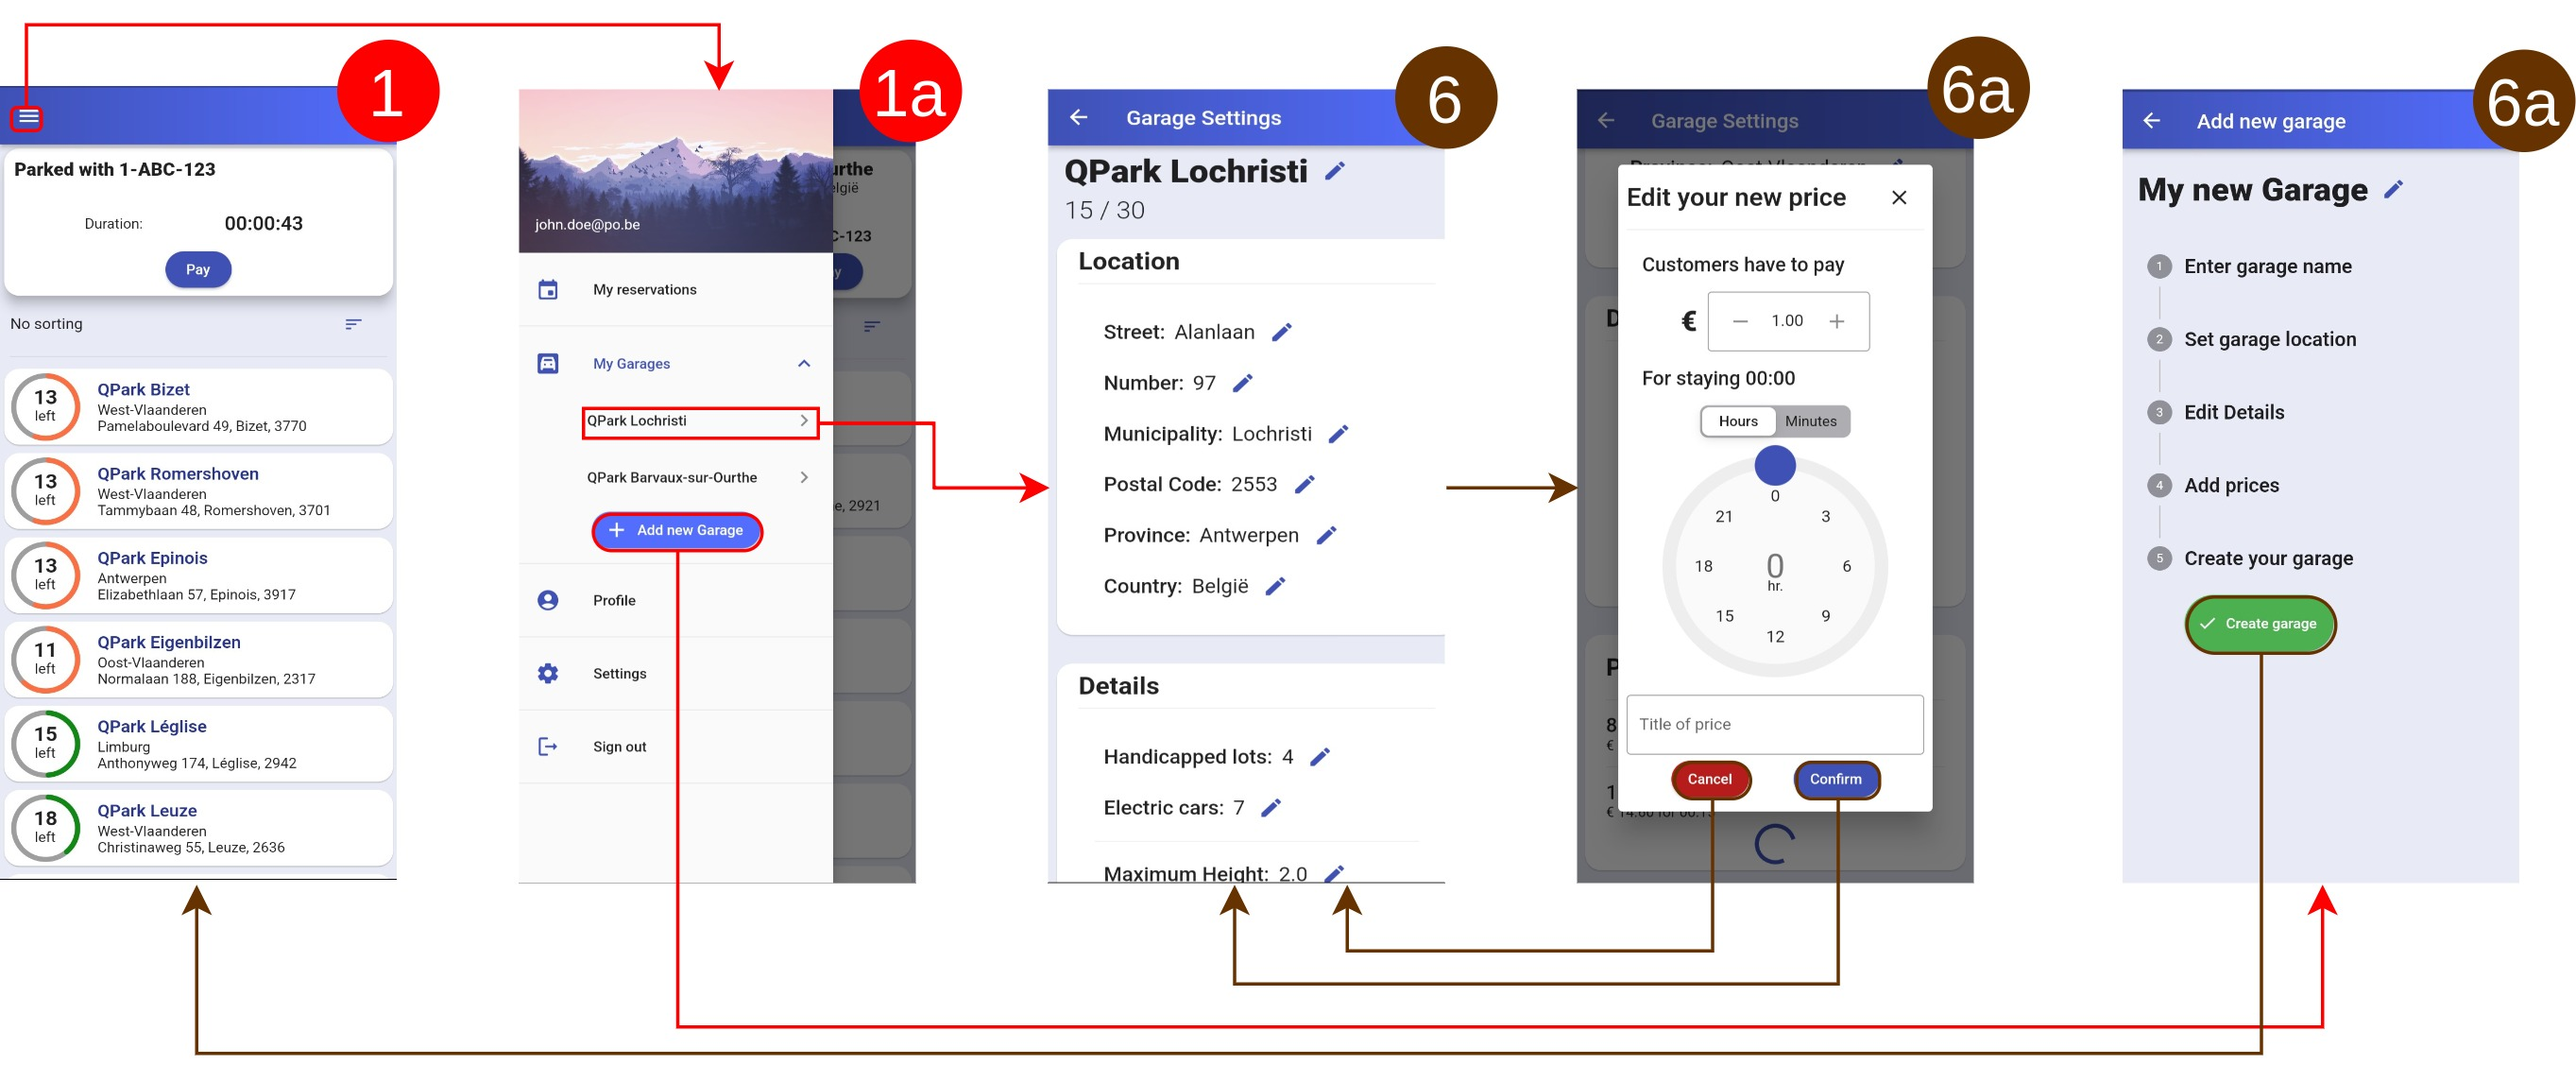
\includegraphics[width=16cm]{images/app/app_diagrams/app_diagram-garage-settings-flow.jpg}
    \caption{App diagram of the garage settings flow (Flow 6).}
   \label{fig:garage-settings-flow}
\end{figure}
\begin{figure}[!hpt]
    \centering
    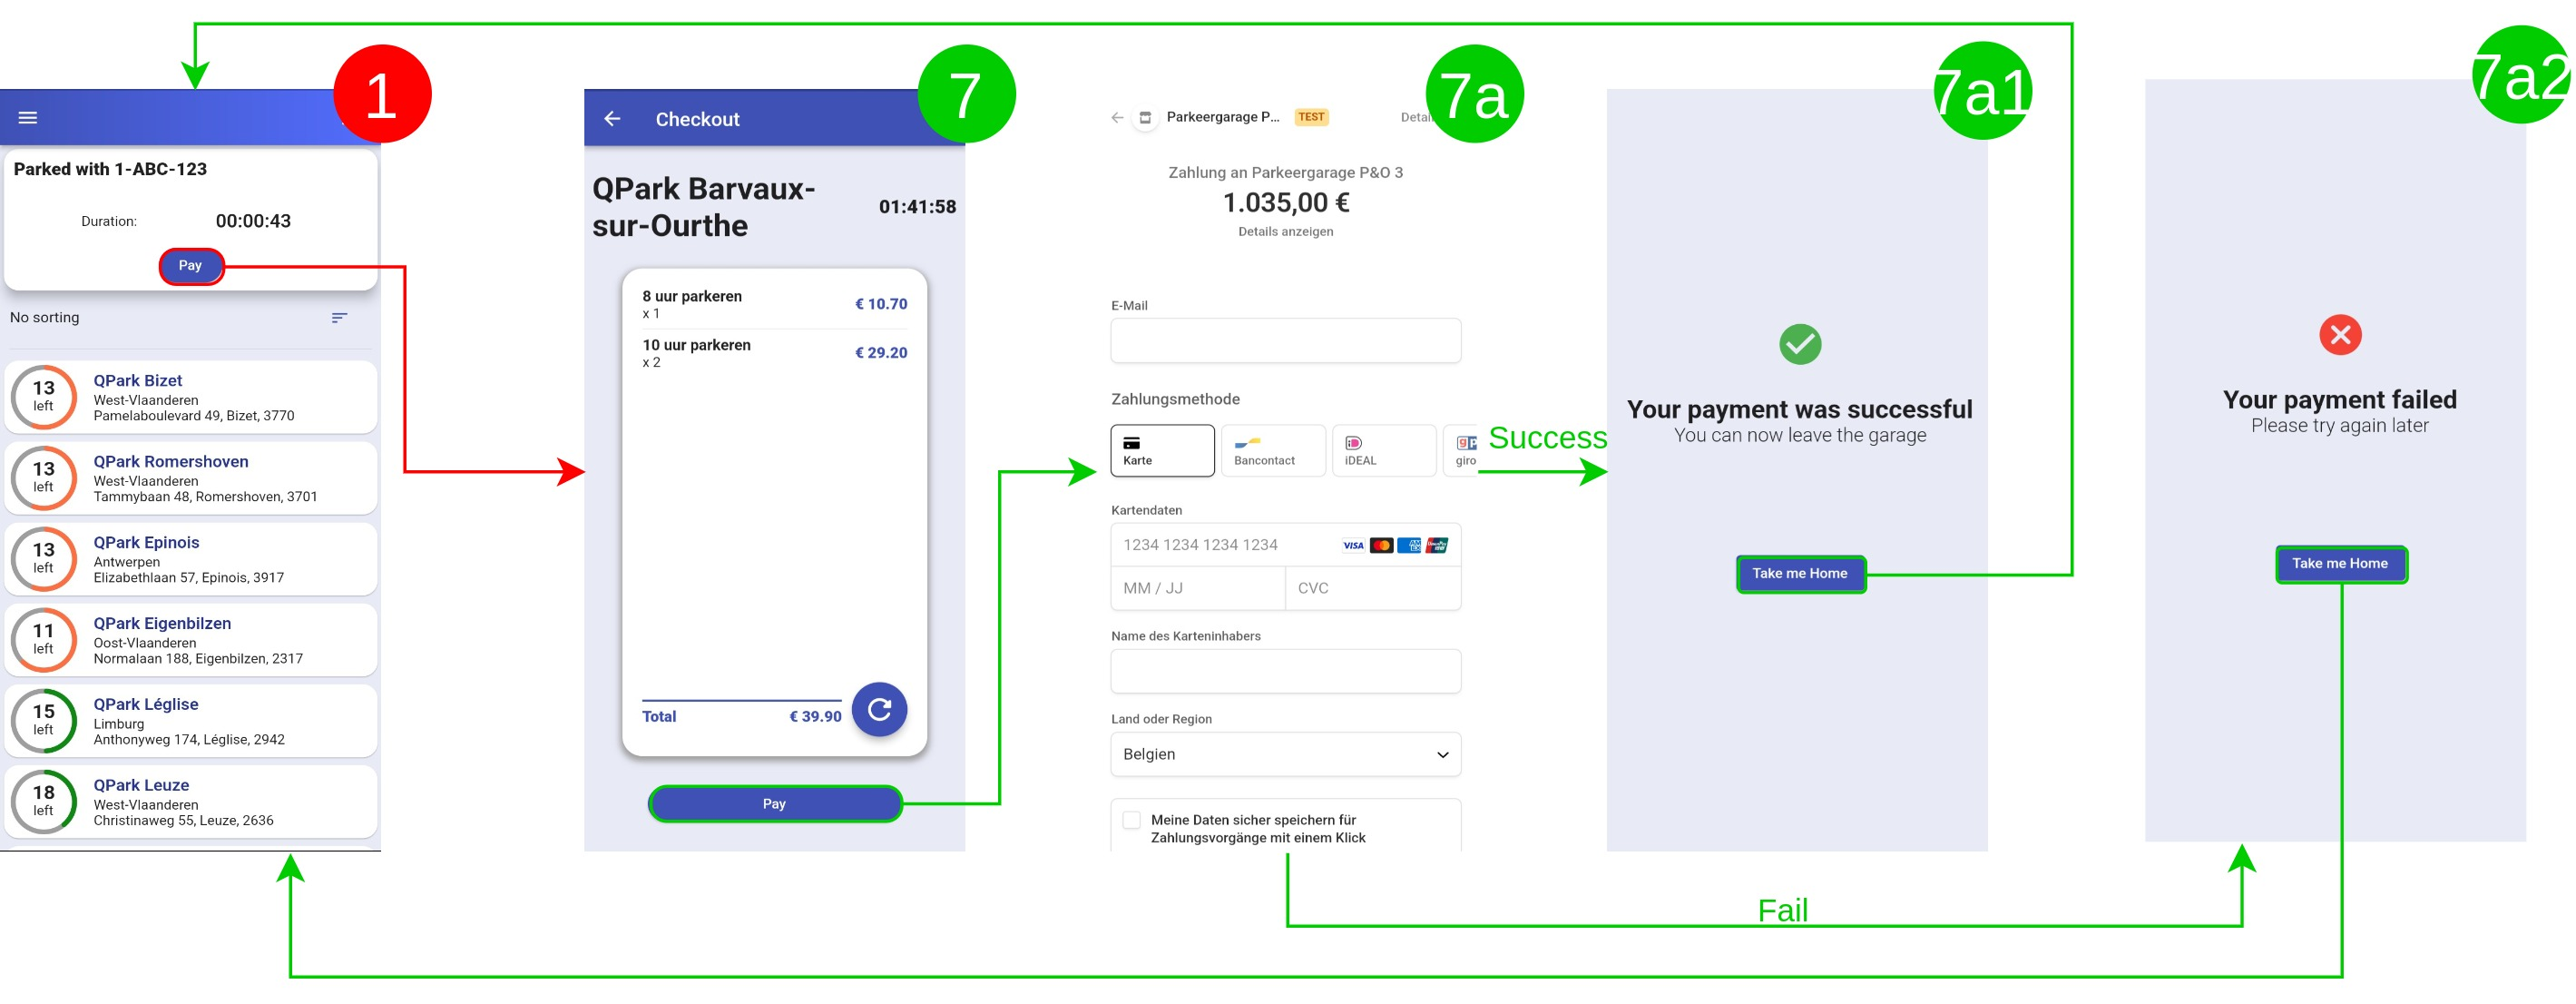
\includegraphics[width=16cm]{images/app/app_diagrams/app_diagram-payment.jpg}
    \caption{App diagram of the payment flow (Flow 7).}
    \label{fig:payment-flow}
\end{figure}

\clearpage

\begin{figure}[htp]
     \centering
     \begin{subfigure}[b]{0.30\textwidth}
         \centering
         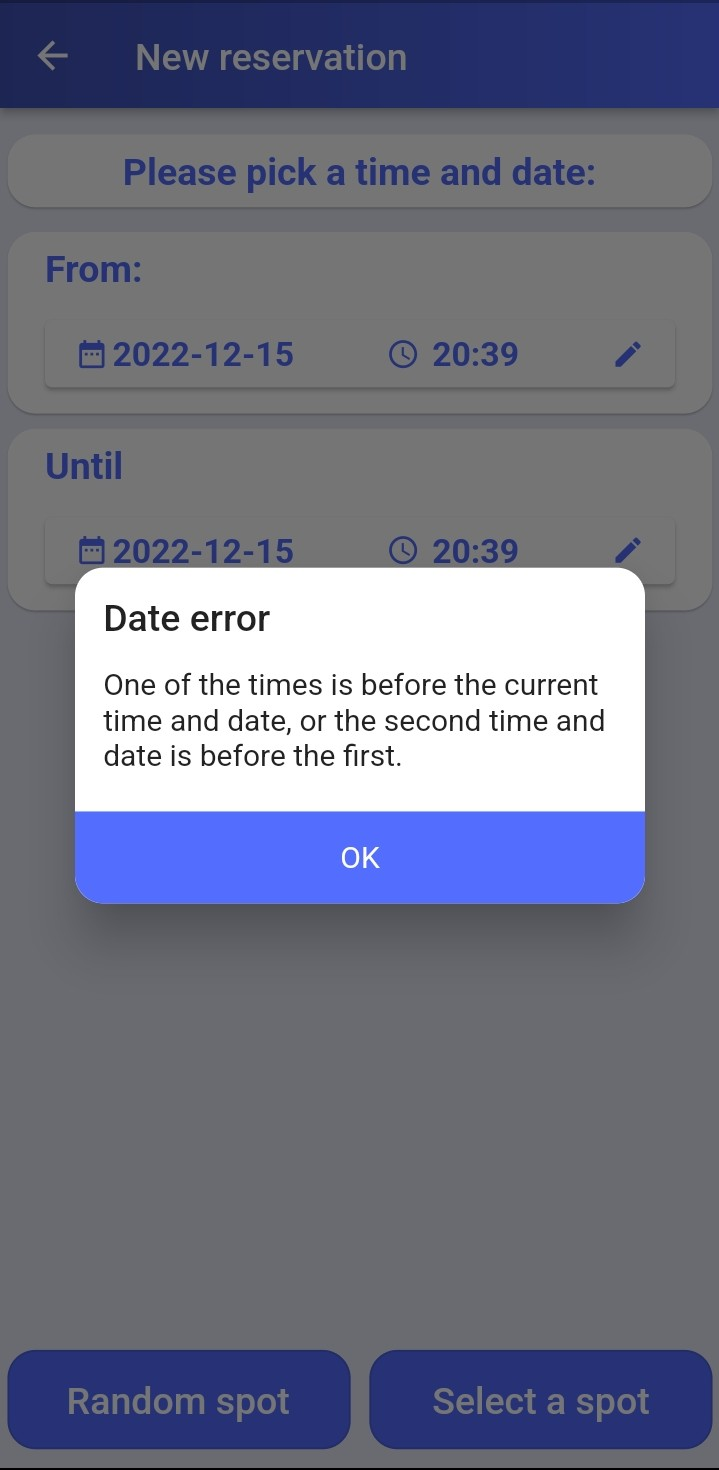
\includegraphics[width=\textwidth]{images/app/dialog1.jpg}
     \end{subfigure}
     \hfill
     \begin{subfigure}[b]{0.30\textwidth}
         \centering
         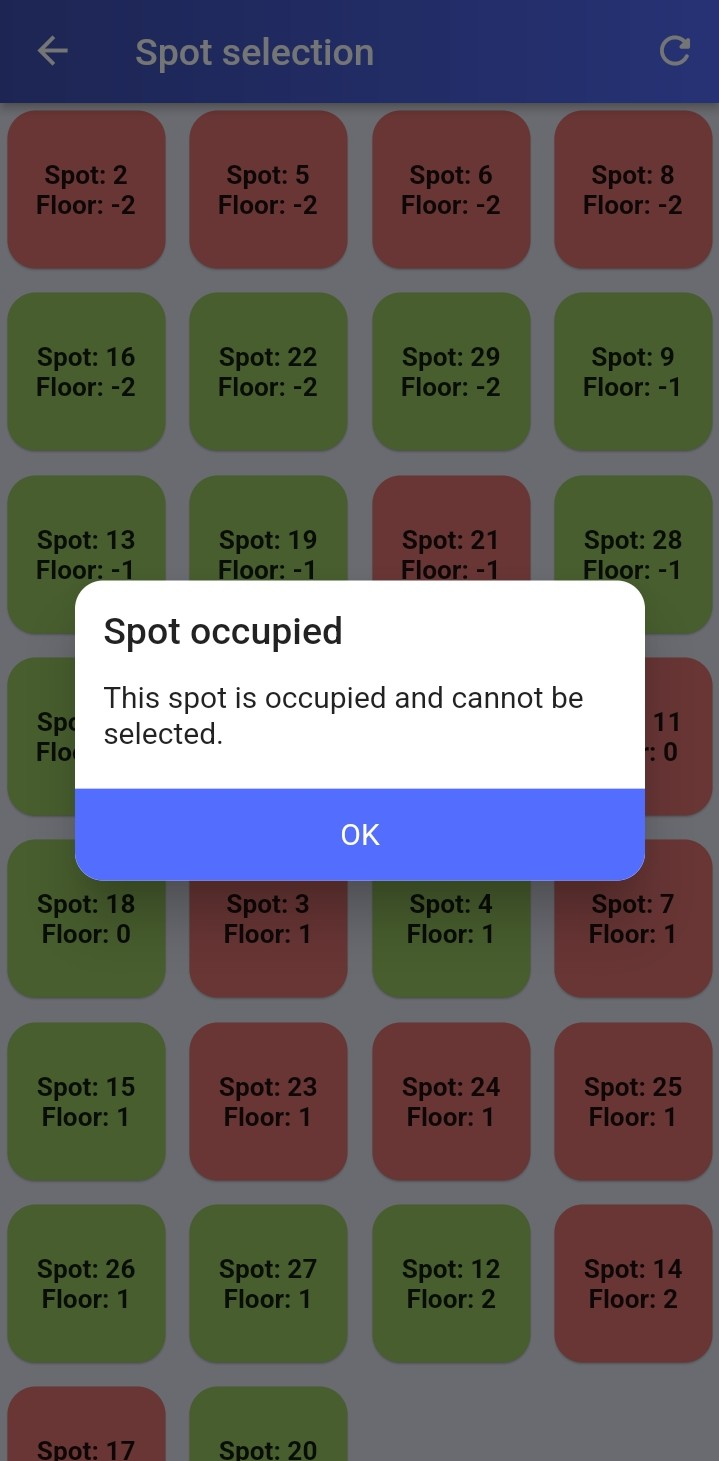
\includegraphics[width=\textwidth]{images/app/dialog2.jpg}
     \end{subfigure}
        \caption{Examples of error pop ups in the frontend application.}
        \label{fig:error-dialogs}
\end{figure}
\begin{figure}[!htp]
     \centering
     \begin{subfigure}[b]{0.30\textwidth}
         \centering
         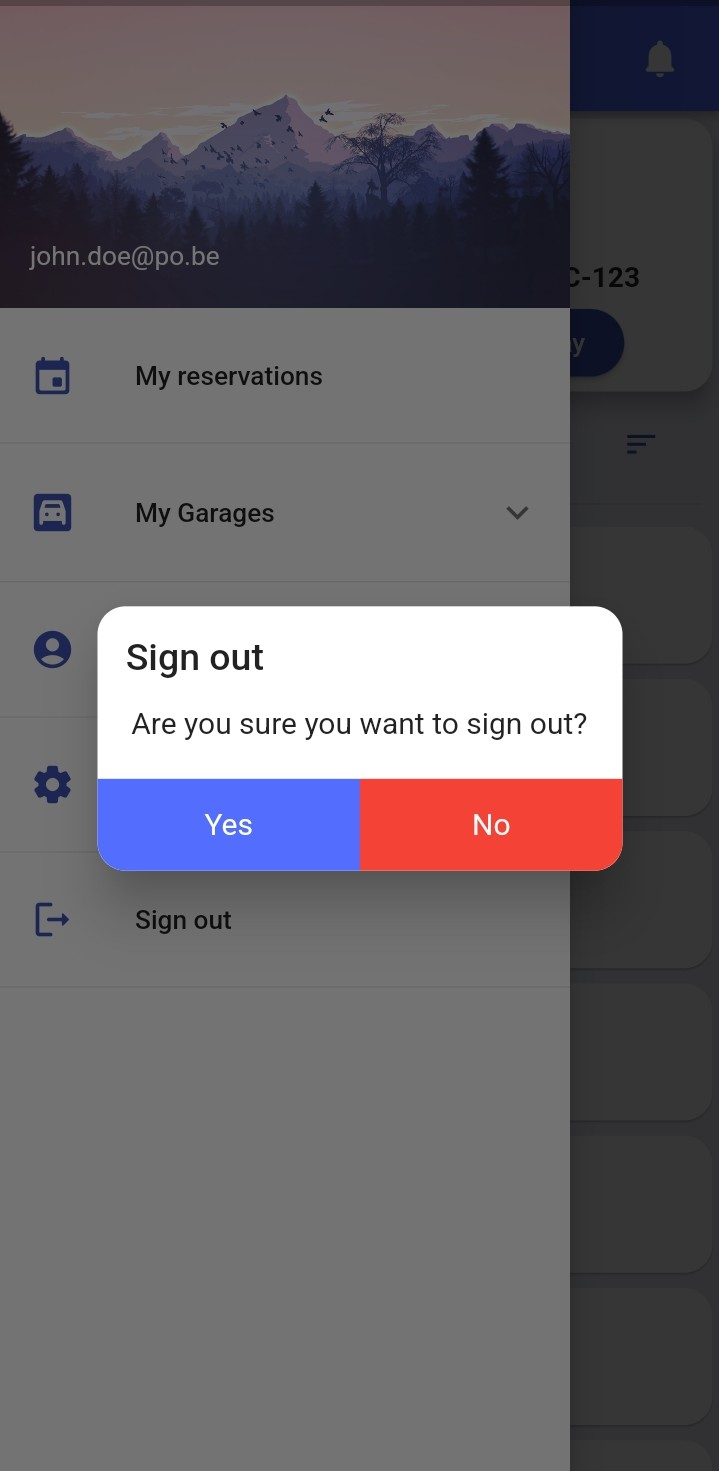
\includegraphics[width=\textwidth]{images/app/dialog3.jpg}
     \end{subfigure}
     \hfill
     \begin{subfigure}[b]{0.30\textwidth}
         \centering
         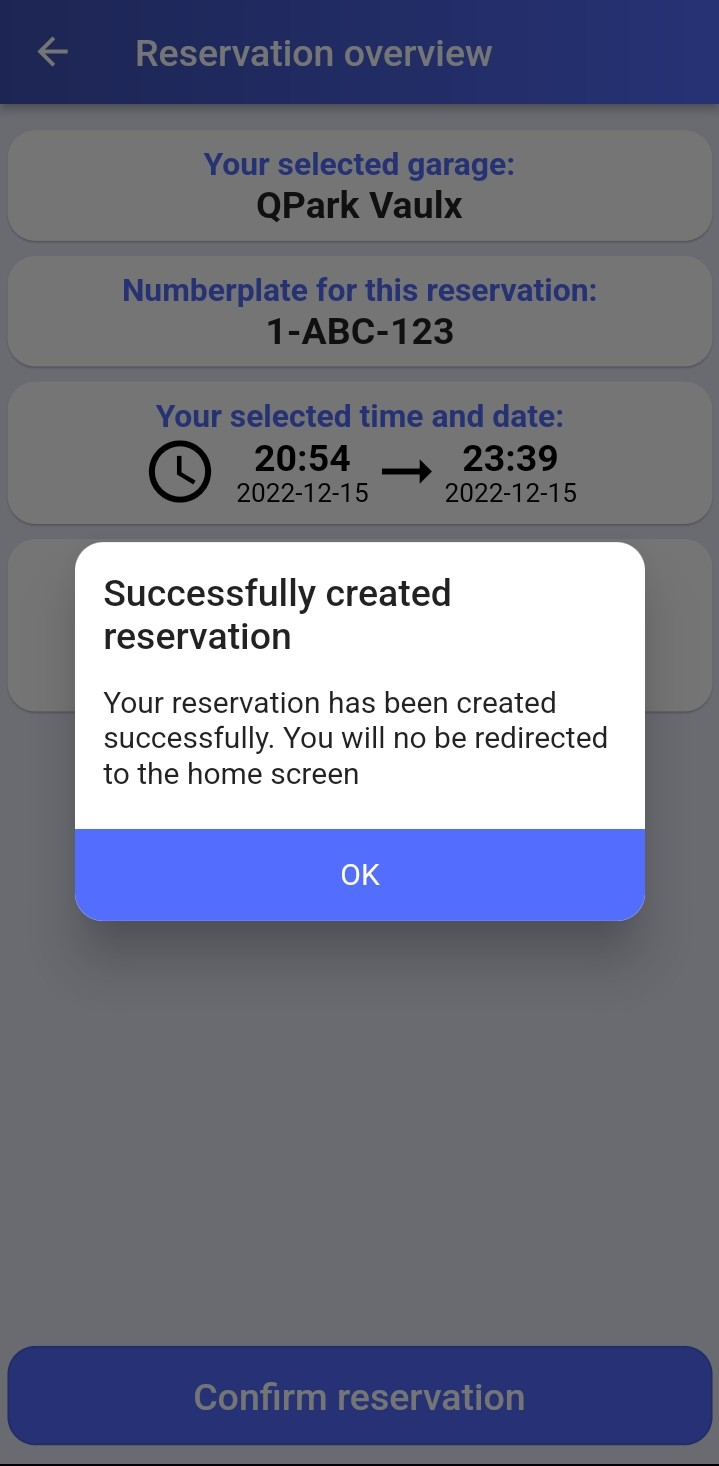
\includegraphics[width=\textwidth]{images/app/dialog4.jpg}
     \end{subfigure}
        \caption{Examples of information pop ups in the frontend application.}
        \label{fig:information-dialogs}
\end{figure}

\clearpage
